% *********************************************************************
% © 2016–2026 Jeremy Sylvestre
%
% Permission is granted to copy, distribute and/or modify this document
% under the terms of the GNU Free Documentation License, Version 1.3 or
% any later version published by the Free Software Foundation; with no
% Invariant Sections, no Front-Cover Texts, and no Back-Cover Texts. A
% copy of the license is included in the appendix entitled “GNU Free
% Documentation License” that appears in the output document of this
% PreTeXt source code. All trademarks™ are the registered® marks of
% their respective owners.
%
% *********************************************************************
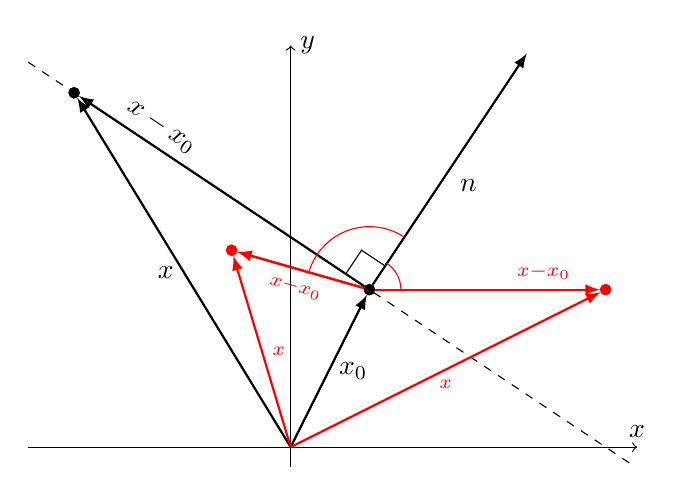
\begin{tikzpicture}[
	point/.style={circle,draw,very thin,fill,inner sep=0pt,minimum size=4pt},
	vector/.style={-latex},
]

	\draw[->] (-3.333,0) to (4.4,0) node[above] {$x$};
	\draw[->] (0,-0.25) to (0,5.1) node[right] {$y$};

	\draw[dashed] (-3.333,4.889) to (4.333,-0.222);
	\node[point] at (1,2) (q) {};
	\node[point] at (-2.75,4.5) (x) {};
	\draw[vector,thick] (q) to node[above,sloped,near end] {$\uvec{x} - \uvec{x}_0$} (x);
	\draw[vector,thick] (q) to node[below right] {$\uvec{n}$} (3,5);
	\draw[vector,thick] (0,0) to node[right] {$\uvec{x}_0$} (q);
	\draw[vector,thick] (0,0) to node[left] {$\uvec{x}$} (x);
	\draw (1.2,2.3) to (0.9,2.5) to (0.7,2.2);

	% some points not on the line
	\node[point,red] at (4,2) (s) {};
	\draw[vector,thick,red] (q) to node[above, sloped, near end] {$\scriptstyle \uvec{x} - \uvec{x}_0$} (s);
	\draw[vector,thick,red] (0,0) to node[below] {$\scriptstyle \uvec{x}$} (s);
	\draw[red] (q) ++(56.3:0.4cm) arc (56.3:0:0.4cm);
	\node[point,red] at (-0.75,2.5) (t) {};
	\draw[vector,thick,red] (q) to (t);
	\draw[vector,thick,red] (q) to node[below, sloped] {$\scriptstyle \uvec{x} - \uvec{x}_0$} (t);
	\draw[vector,thick,red] (0,0) to node[right] {$\scriptstyle \uvec{x}$} (t);
	\draw[red] (q) ++(56.3:0.8cm) arc (56.3:164.05:0.8cm);

\end{tikzpicture}
